\documentclass[24 pts]{article}
\usepackage{xeCJK}
\usepackage{amssymb}
\usepackage{amsmath}
\usepackage{amsthm}
\usepackage{graphicx}
\graphicspath{ {images/} }
\usepackage{relsize}

\newcommand{\me}{\mathrm{e}}
\setCJKmainfont[BoldFont= Yu Mincho Demibold]{MS Mincho}
\title{情報・ネットワーク工学選考基礎 レポート }
\date{04-08-2016}
\author{Kwame Ackah Bohulu 1631133}
\begin{document}
\maketitle
\section{Cellular Automaton}
A cellular automaton (CA) is a collection of "colored" cells on a grid of specified shape that evolves through a number of discrete time steps according to a set of rules based on the states of neighboring cells. The rules are then applied iteratively for as many time steps as desired.
\subsection{Mathematical Definition}
%The states of the automaton come from a finitestate set S. At any given time, the configuration of the automaton is a mapping $c:\mathbb{Z}^d\mapsto S$ that specifies the states of all cells. TheLet $N =(\overrightarrow{x_1},\overrightarrow{x_2},...,\overrightarrow{x_n})$ be distinct elements of $\mathbb{Z}^d$. Then the neighbours of a cell at location $\overrightarrow{x}\in \mathbb{Z}^d$ are the n cells at location $$ \overrightarrow{x}+\overrightarrow{x_i}$$ for $i=1,2,...,n$%

 A
d-dimensional CA is specified by a triple
(S,N,f)
where
S is the state set,
$N\in(S^{\mathbb{Z}^d})^n$
is the neighborhood vector, and
$f:S^n\mapsto S$
is the local update rule. We usually identify a CA with its global transition function
$G:C\mapsto C$
, and
talk about CA function
G
, or simply CA
G.
The set $S^{\mathbb{Z}^d}$ of all configurations is denoted by
$C
(d,S)$
, or briefly C
when
d
and
S
are known
from the context. Constant functions are called
homogeneous
configurations.
The cells change their states synchronously at discrete time steps. The next state of each
cell depends on the current states of the neighboring cells according to an update rule. All
cells use the same rule, and the rule is applied to all cells at the same time. The neighboring cells may be the nearest cells surrounding the cell, but more general neighborhoods can
be specified by giving the relative offsets of the neighbors.
\subsection{Examples for d=1}
\subsubsection{rule 90}
For simplicity sake, the case of a one dimensional CA is considered. it is made up of a line of cells.
\begin{center}
\begin{tabular}
{|c | c || c  | c | c || c | c | c | c | c | }
\hline
1 & 0 & 1 & 0 & 1 & 1 & 1 & 0 & 0 & 1 \\
\hline
\end{tabular}
\end{center}
The state set $S =\{0,1\}$\\
The neighbourhood vector size is $2^3=8$ and the neighbourhood vector N is given by $$\{000,001,010,011,100,101,110,111\}$$
The local update rule, f is given by 
$$\{000\mapsto 0,001\mapsto 1,010\mapsto 0,011\mapsto 1,100\mapsto 1,101\mapsto 0,110\mapsto 1,111\mapsto 0\}$$
This decision rule is known as \textit{rule 90} because 01011010 is the binary representation of the decimal number 90.Assuming the edges to be constant, the table below shows the next 2 states after the initial states. 
\begin{center}
\begin{tabular}
{|c | c | c  | c | c | c | c | c | c | c | }
\hline
1 & 0 & 1 & 0 & 1 & 1 & 1 & 0 & 0 & 1 \\
\hline
1 & 0 & 0 & 0 & 1 & 0 & 1 & 1 & 1 & 1 \\
\hline
1 & 1 & 0 & 1 & 0 & 0 & 1 & 0 & 0 & 1 \\
\hline
\end{tabular}
\end{center}
After a number of updated and setting 0=white and 1 =black, we get the figure below\\
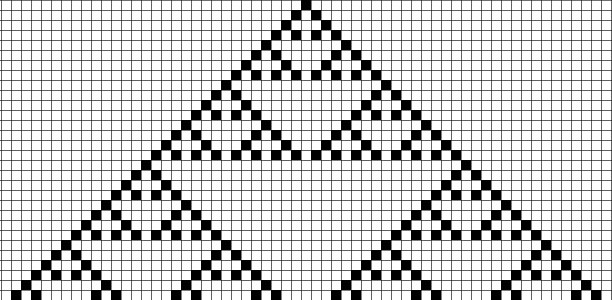
\includegraphics[scale =0.3]{Rule90}\\
\subsubsection{rule 222}
in this case, the local update rule, f is given by 
$$\{000\mapsto 1,001\mapsto 1,010\mapsto 0,011\mapsto 1,100\mapsto 1,101\mapsto 1,110\mapsto 1,111\mapsto 0\}$$. After a number of state updates, we get the figure below.\\ 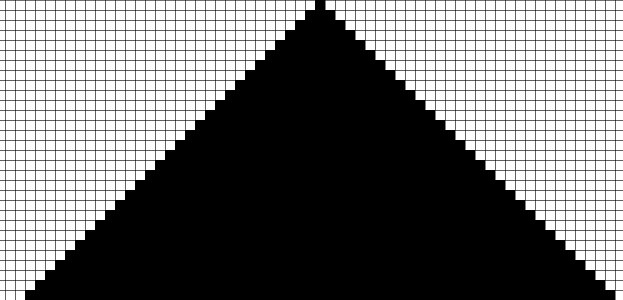
\includegraphics[scale =0.5]{Rule222}\\
There is also the popular 2-dimensional CA known as the "Game of Life" which has more complex update rules and a larger size neighbourhood vector.
The rules of the Game of Life are given below.\\


    [1].Death. If a cell is alive (state = 1) it will die (state becomes 0) under the following circumstances.
\paragraph{}
        [a].Overpopulation: If the cell has four or more alive neighbors, it dies.
\paragraph{}
        [b].Loneliness: If the cell has one or fewer alive neighbors, it dies.\\

    [2]Birth. If a cell is dead (state = 0) it will come to life (state becomes 1) if it has exactly three alive neighbors (no more, no less).\\

    [3]Stasis. In all other cases, the cell state does not change. To be thorough, let’s describe those scenarios.
\paragraph{}
        [a]Staying Alive: If a cell is alive and has exactly two or three live neighbors, it stays alive.
\paragraph{}
        [b]Staying Dead: If a cell is dead and has anything other than three live neighbors, it stays dead.

\subsection{Cellular Automaton Research Areas}
\paragraph{Computer Processors}
Cellular automaton processors are physical implementations of CA concepts, which can process information computationally. Processing elements are arranged in a regular grid of identical cells. The grid is usually a square tiling, or tessellation, of two or three dimensions; other tilings are possible, but not yet used. Cell states are determined only by interactions with adjacent neighbor cells. No means exists to communicate directly with cells farther away.One such cellular automaton processor array configuration is the systolic array. Cell interaction can be via electric charge, magnetism, vibration (phonons at quantum scales), or any other physically useful means. This can be done in several ways so no wires are needed between any elements. This is very unlike processors used in most computers today, von Neumann designs, which are divided into sections with elements that can communicate with distant elements over wires.
\subsection{References}
1. Daniel Shiffman, "The Nature of Code", Chapter 7\\
2. https://en.wikipedia.org/wiki/Cellular\_automaton\\
3. Wolfram,Stephen.
"A New
Kind
of Science"
. Champaign,
IL: Wolfram
Media
Inc.,
2002\\
4. Jarkko Kari,"Theory of cellular automata :A survey",Theoretical Computer Science 334 (2005) 3 – 33
\end{document}